\chapter{Gap Reconstruction}
\label{Sec:GapFill}
One of the more common problems in citizen science projects is gaps in data. This can happen either if the network connection is unstable or the test equipment gets prematurely turn off, as discussed in chapter \ref{Sec:DataQuality}. This can greatly degrade the data quality, and lead to errors in the application. One way to deal with this problem is to use mathematical gap filling techniques to come with a qualified guess on how the data would look like in the gap. 

In order to use this methods we must assume that the missing data in the gap follows the same behaviour as the data on each side off the gap. If the signal is so stochastic that this is not the case then gap filling is not recommended\citep{RefWorks:10}. 

In the case of the SmartHG project the data can be seen to have a part that is depended on the previous and future data plus a stochastic part that are determined by the user and the appliance. Due to the stochastic part a perfect reconstruction is not possible, but it is the hypotheses that the non stochastic part is still so dominant that a decent reconstruction is possible. 

\section{Gap Filling Methods}
\label{T:GapFilling}
Various methods exists for gap filling. Five popular algorithms are selected for this project, and is validated on the SmartHG project data. These methods have been chosen since they all have a different approach on the gap filling process. For some of the algorithms it is important to keep the frequency spectra as intact as possible, for other it is the jitter power or the exact sample value they are trying to estimate. Some algorithms have also been designed for small gaps, while others have been designed for larger. 

In the following sections it will be briefly described what makes the five algorithms unique, and how they work. 

\subsection{Papoulis-Gerchberg Algorithm}
\label{T:PGA}
The \ab{P-G}[Papoulis-Gerchberg] algorithm is a multi gap filling algorithm, meaning it is capable of correcting more than one gap at the time. This makes the algorithm preform good in conditions with many gaps and few available data points between gaps. This is due to its ability to collect information about the signal across multiple gaps\citep{RefWorks:11}. The \ab{P-G} algorithm works under the assumption that the signal is a periodic stationary signal with a known bandwidth. The signal will therefore consist of $M$ frequency components, and everything outside the band is assumed to be noise. The signals in the SmartHG is not stationary, but for small snippets can approximately stationariness be assumed. 

The true bandwidth is also unknown in the signal. The \ab{P-G} algorithm is very depended on the bandwidth for a correct reconstruction. A modified version of the algorithm that estimates the bandwidth, by varying the frequency components $M$ and analysing the mean square error on the known signal is therefore used \cite{RefWorks:13}. This approach is fairly good at estimating the true value of $M$, but it is time-consuming.

\subsection{Wiener Filling Algorithm}
The Wiener filling algorithm is an extension of a Wiener predictor, the Wiener predictor assumes that there exist a linear relationship between the next sample and the previous samples. By trying to predict the missing samples from both sides of the gap, and combining the knowledge, it estimates the missing samples \citep{RefWorks:14}. For larger gaps does this methods rely on earlier predictions to close the gaps. This result in errors being accumulated over the gaps. The method is fast, and is therefore suited for large data with small gaps. 

\subsection{Spatio-Temporal Filling Algorithm}
The \ab{SSA}[Spatio-Temporal filling] algorithm uses singular spectrum analysis to split the signal into a series of sub-signals. The sum of the sub-signals is the original signal, and the sub-signals are ordered so the most dominant is first, and the least dominant is last. 

The reconstruction philosophy is that the gap has introduced noise in the signal, but a sum of only the most dominant sub-signals must be close to the original signal without noise. But in order to know how many sub-signals to include in this sum, we introduce an other artificial gap. While the sub-signals are being accumulated the mean square error of the artificial gap is observed. When this mean square error hits its minimum peek, it is assumed that the reconstruction is as good as possible \cite{RefWorks:15}.

This method is very popular for gap filling. It has shown to be very noise resistant since it finds the overall trends in the data. It does require quite a lot of data to be known post and prior to the gap since an artificial gap must be introduced. It is based on singular spectrum analysis which assumes that the signal consist of stationary processes. This is a similar constraint to the \ab{P-G} Algorithm in section \ref{T:PGA}.

\subsection{Envelope Filling Algorithm}
\label{T:EGA}
Unlike the previous described methods does the Envelope filling algorithm not depend on frequency analyses, but rather on the expected power of the signal. Looking at the envelope of the signal it assumes that all local maxima and minima must lie on the  upper and lower envelope. It then looks at the data prior and post the gap and try to estimate the number of local maxima and minima in the gap, and their locations. It does this by looking for patterns in the time series data \citep{RefWorks:6}. When the new maxima and minima are found the points is connected by using spline \cite{RefWorks:16}. 

The methods do not make any assumptions about the signals stationariness or bandwidth. The method can also be used on none equally spaced time series. 

\subsection{Empirical Mode Decomposition Filling Algorithm}
The \ab{EMD}[empirical mode decomposition filling] algorithm uses empirical mode decomposition, to break the signal into \ab{IMF}[intrinsic mode functions]. The sum of all \ab{IMF}'s is the original signal. The \ab{IMF}'s is all more low frequent and simpler in structure than the original signal. The hypothesis is that it is easier fixing a gap in a simple signal than a complex one. 

The envelope filling algorithm in section \ref{T:EGA} is used to fix the gaps in the \ab{IMF}'s. The \ab{IMF}'s can now be accumulated to get the original fixed signal. Like the envelope filling algorithm does it not make any assumptions about the signals stationariness, bandwidth and can be used on none equally spaced time series. But making a empirical mode decomposition on a signal with a gap in is a non trivial process and can introduce errors \citep{RefWorks:16}. 



\section{Gaps In SmartHG Dataset}
The gaps in the SmartHG project dataset is caused by a lot of different sources such as bad network connection, unplugged measurement equipment or server breakdown. This makes the type of gaps different from case to case. Three aspects of a gap is important for the gap filling: The size of the gap, the data known before the gap, and the data known after the gap. 

\subsection{Gap Size}
On figure \ref{fig:GapSize} is the quantity of different gaps shown. The different gap size is measured as samples missing, e.g. a gap size on 3 means that there is 3 samples missing in a row, between two received samples. Looking at the different gaps in the dataset we see that the normal gap is relatively small. Most of the gaps are between 1-5 samples as seen figure \ref{fig:GapSize}.

\begin{figure}[H]
\centering
\begin{minipage}{.3\textwidth}
  \centering
  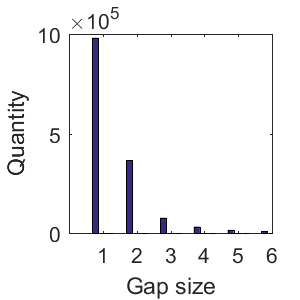
\includegraphics[width=1\linewidth]{billeder/GapInfo1.png}
  \captionof{figure}{Gap quantity}
  \label{fig:GapSize}
\end{minipage}%
\begin{minipage}{.8\textwidth}
  \centering
  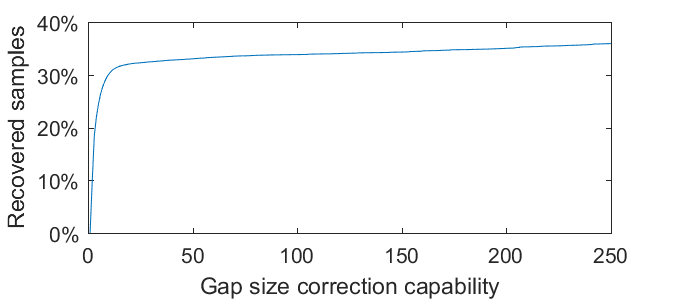
\includegraphics[width=0.8\linewidth]{billeder/CorrectionCapability.png}
  \captionof{figure}{Error recovery capability}
  \label{fig:GapCorrect}
\end{minipage}
\end{figure}

The aim of data reconstruction is to recover the missing samples. The gap size correction capability is a metric telling how big gaps it is possible to correct. If a application has a gap size correction capability on 5 it means that is is capable of correcting gaps that have the gap size of 5 samples or smaller. 

On figure \ref{fig:GapCorrect} is shown how much of the missing signal that can be reconstructed with different gap size correction capability. It is shown that a if a gap size correction capability of approximately 20 samples can be achieved, it is possible to recover $30\%$ of the missing data in the SmartHG dataset. Since the signal is partly stochastic, and it is not possible to recover the stochastic part, the complete signal can newer be reconstructed. The greater the gap, the greater influence does the stochastic part have on the signal. Smaller gaps can therefore be fixed with greater success. It is therefore unlikely that recovery of more than $30\%$ will be possible. 

\subsection{Post And Prior Knowledge}
The reconstruction process works by looking at the samples available prior and post of the gap. Common for all reconstruction methods is that they assume that the signal in the gap must have behaved in relation to the samples prior and post for the gap. Therefore is the samples prior and post for the gap called knowledges, since it grants the knowledges used for reconstructing the gap. 

But in a signal with lots of gaps it can be interesting to see how much knowledge is available for reconstructing a gap. This is done by seeing how many samples that are available prior and post to the gap. This is important since much data allows for detailed models, that can improve gap reconstruction and little knowledge gives the stochastic part dominance which will lead to error prone reconstruction. 

\begin{figure}[H]
\centering
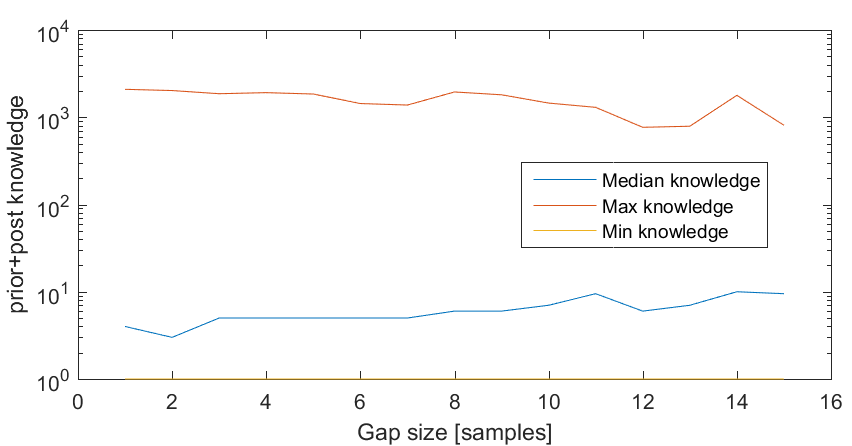
\includegraphics[width=0.7\linewidth]{billeder/GapInfo2.png}\caption{Available samples for recovery}
\label{fig:PAF}
\end{figure}

In the case of the SmartHG project dataset the data available prior and post to a gap varies greatly but is around the same max and min values for every gap size. The median samples available to fix a gap is around 6 samples as shown in figure \ref{fig:PAF}. On the figure is shown that no matter the gap size is the expected knowledge about the same. This can be problematic since lager gaps offend needs more knowledge than smaller gaps. This further indicates that complete recovery of all gaps is impossible. 

\section{SmartHG Dataset Reconstruction}
The data reconstruction algorithms mentioned on section \ref{T:GapFilling} have been tied on the SmartHG dataset. First have 6 unique error free areas in the data been found, and a artificial gap have been introduced in the 6 scenarios. 
The gaps have now been reconstructed, and a comparison to the true value is made. 

The 6 scenarios have been randomly chosen under the constraints that there where no missing data in them, and they all are different in activity level from the other chosen scenarios. Both accumulative scenarios and non accumulative scenarios have been chosen. 

There are several ways of comparing the different algorithms, in this report 3 have been selected based on the likelihood of the importance in a learning algorithm, which is the target application for the data. The first is a simple sample by sample comparison, where it is seen how much each sample differs from the true value. The other is the frequency, where it is analysed how much the frequency response is different. The last is a method called jitter compression, where we see that the power of the jitter is the same, more on this in section \ref{T:jitterCom}.

\subsection{Sample Comparison}
The sample by sample comparison is created by finding the mean square error of the samples compared to there true values.  

\begin{figure}[H]
\centering
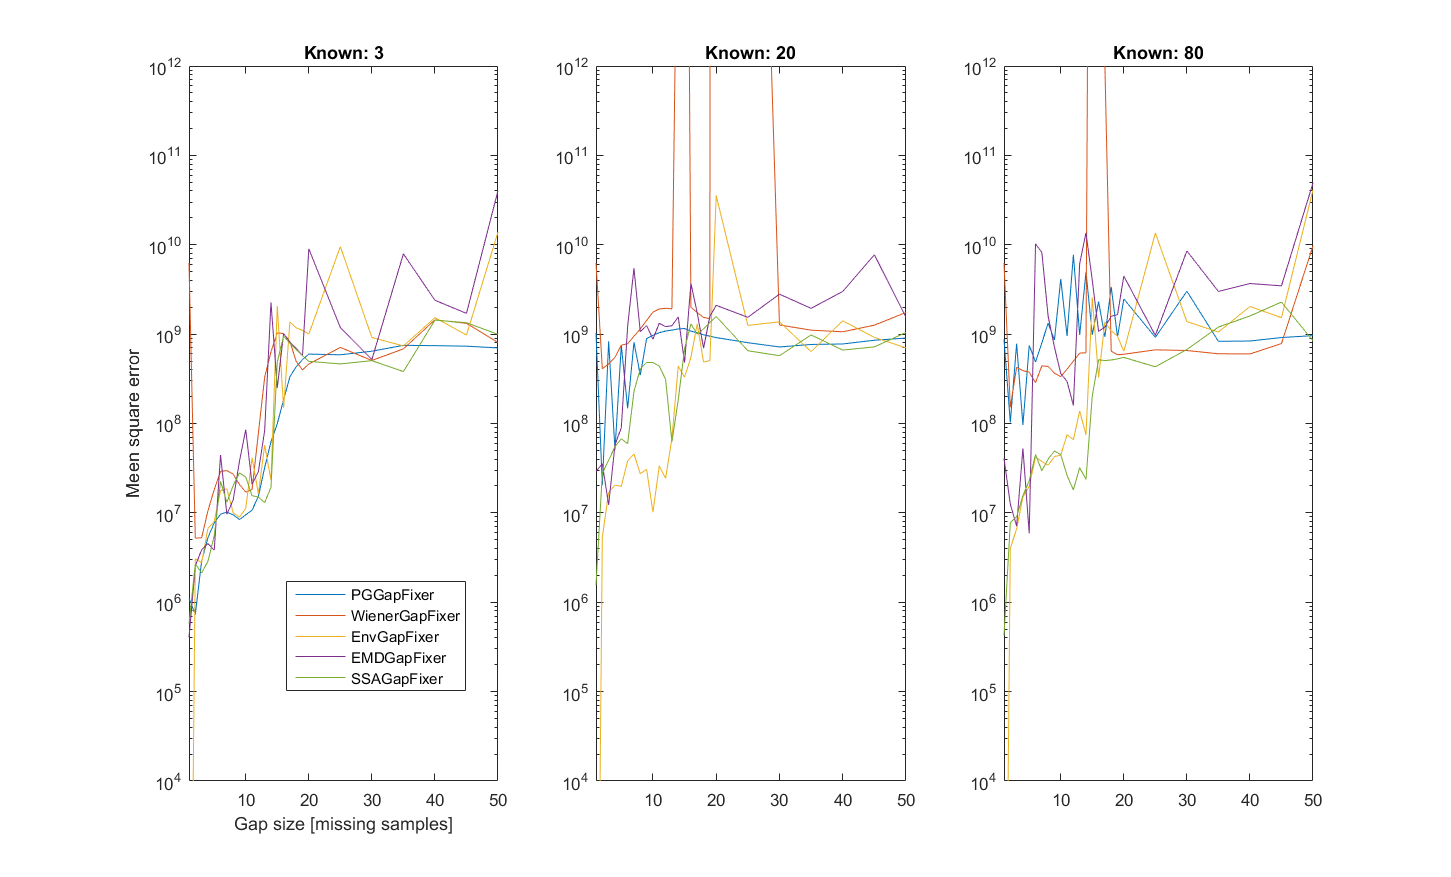
\includegraphics[width=1\textwidth]{billeder/RecNorm.png}
\caption{Sample comparison of the reconstruction methods}
\label{fig:RecNorm}
\end{figure}

On figure \ref{fig:RecNorm} is the result shown for 3 different cases. The Known attribute indicates how much prior and post knowledge in samples is used to reconstruct the gap. On the x axis is shown the gap size, as expected does the prediction grow worse the greater the gap size. As a baseline is a linear predictor also added. The linear predictor makes a simple line between the two samples at each edge of the gap, and places all missing samples on the line. 

As seen on the figure the best reconstruction is made by the \ab{P-G} algorithm, with relatively few samples as knowledge. The wiener algorithm is also close to the linear base line. The logical statement is the more information or knowledge we have the better should the prediction become. This does not seems to be the case, since a lot of the algorithms amperes to preform better at lower knowledge rate. This can be explained by the stochastic part of a signal, when the knowledge is small it is more likely that the information around the gap is relevant, the more knowledge grows the more likely is it the a stochastic event will bring false information to the model. This can be illustrated as on figure \ref{fig:StocIls}.

\begin{figure}[H]
	\begin{picture}(300,200)
	\put(0,0){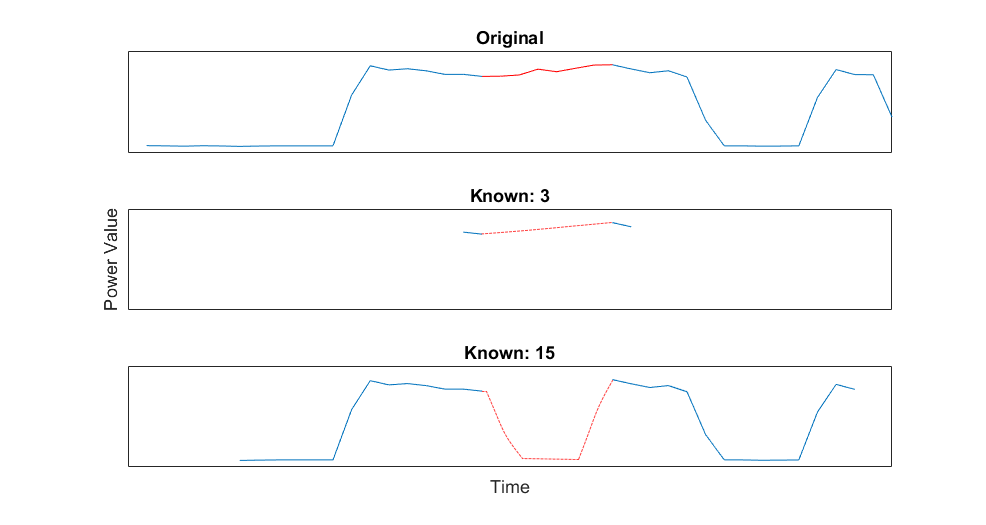
\includegraphics[width=1\textwidth]{billeder/StocIlustation.png}}

	\put(315,65){Stochastic event}
	\put(365,65){\color{black}\vector(1,-1){10}}
	
	\put(315,210){Stochastic event}
	\put(365,210){\color{black}\vector(1,-1){10}}

	\end{picture}
\caption{Stochastic effect on prediction.}
\label{fig:StocIls}
\end{figure}

On the figure \ref{fig:StocIls} is shown a original signal with a gap, indicated by the red area. The true value is illustrated by the full red line in the original signal. The two subsequent graphs is the reconstruction, the blue area is the known area and the dotted red line is the predicted values. When the known area is small there is not enough frequency information to make any grant changes, so the prediction will look more or less like a linear interpolation. This is compared to the true value not a bad guess. When there is more samples known we are able to make more complex estimates of the signal. On the figure it is shown how when we have a knowledge of 15 we also see the stochastic event. Taking this in to the model, changes the prediction to a less correct value, due to the frequency's added by the stochastic event. 

Since the results shown in figure \ref{fig:RecNorm} at higher knowledge shows that the reconstruction methods for the most part preforms worse than the linear basecase, we can conclude that the signal is quite stochastic and not as periodic as one would hope. For many smart-meters it is possible to get both the instantaneous current power and accumulated power over time as the samples. By looking at the accumulated power before and after a gap it is possible to gesture about the changes in power during the gap. This information can be used to further improve the gap filling. 

\newpage

\subsection{Frequency Comparison}
An other metric to compare is how well the frequency response is preserved in the reconstruction, since this is often more important that the true value itself for smaller devices whit many states like computers. Such devices is often recognised by there usage pattern and not the true power draw. By looking at the Fourier transform of the original signal and the reconstructed power of the different frequencies was compared. 

\begin{figure}[H]
\centering
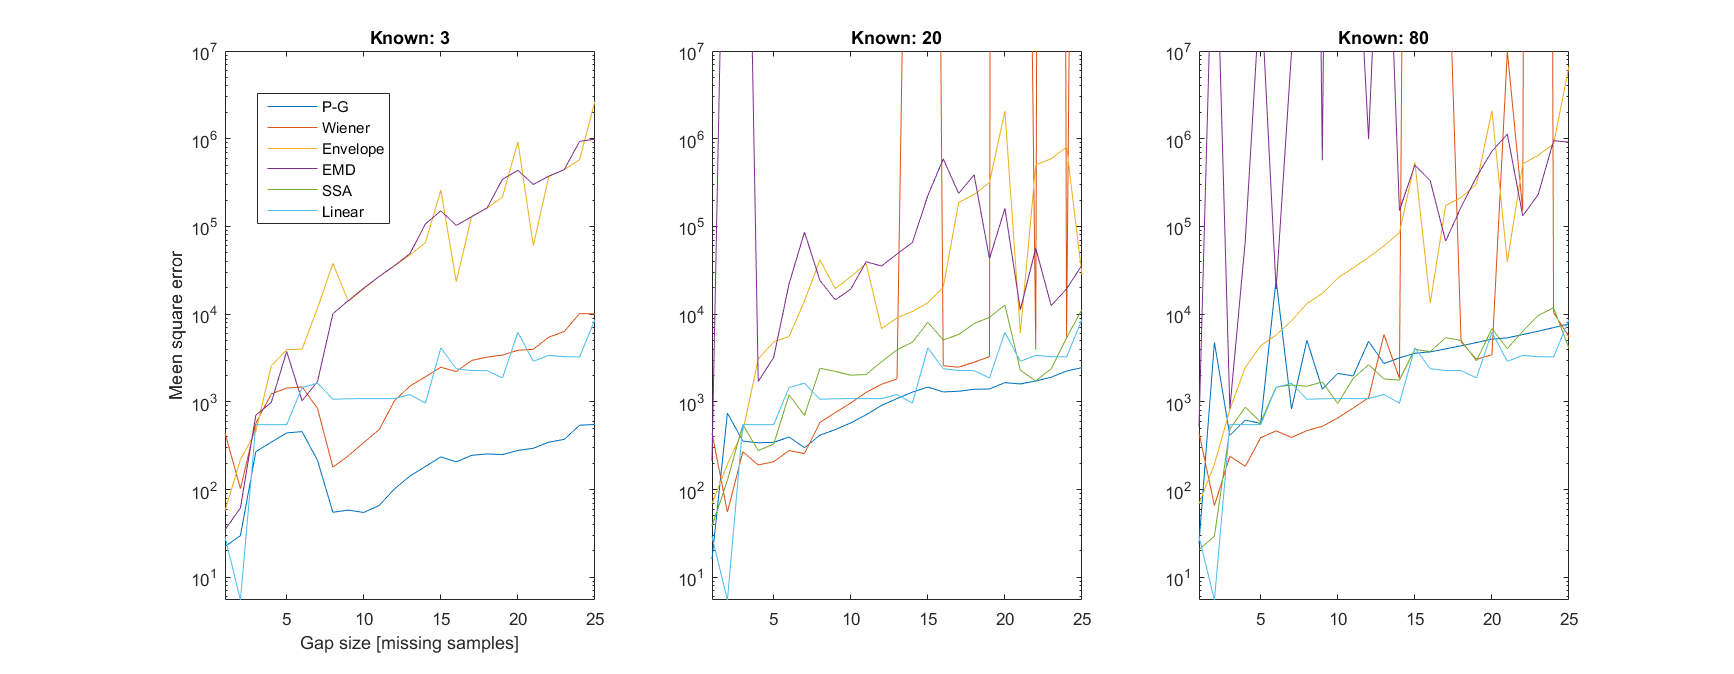
\includegraphics[width=1\textwidth]{billeder/RecFeq.png}
\caption{Frequency comparison of the reconstruction methods}
\label{fig:RecFeq}
\end{figure}

As shown on figure \ref{fig:RecFeq} both the Wiener and the \ab{P-G} Algorithm seems to preform well. Like for the sample comparison the most successful reconstruction seems to be at low knowledge. 

\subsection{Jitter Comparison }
\label{T:jitterCom}

The jitter is a different metric as it tells how well we have modelled the "noise" of the signal. In a jitter analysis the signal is thought of as a slowly changing signal with a faster noise signal embedded in it.

The slow signal is assumed to be found by taking a low pass filter over the signal to filter out the noise. The jitter analysis measures the power in the jitter from this signal as illustrated on figure \ref{fig:JitPow}. 

\begin{figure}[H]
\centering
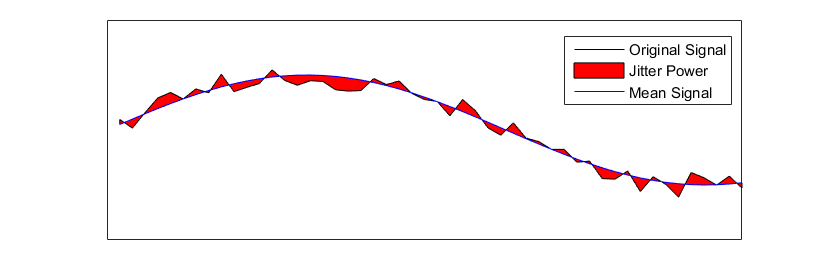
\includegraphics[width=0.7\textwidth]{billeder/JitterPower.png}
\caption{Jitter Power Illustration}
\label{fig:JitPow}
\end{figure}

It the estimated jitter power have been compared with the real jitter power for all the reconstruction methods. 

\begin{figure}[H]
\centering
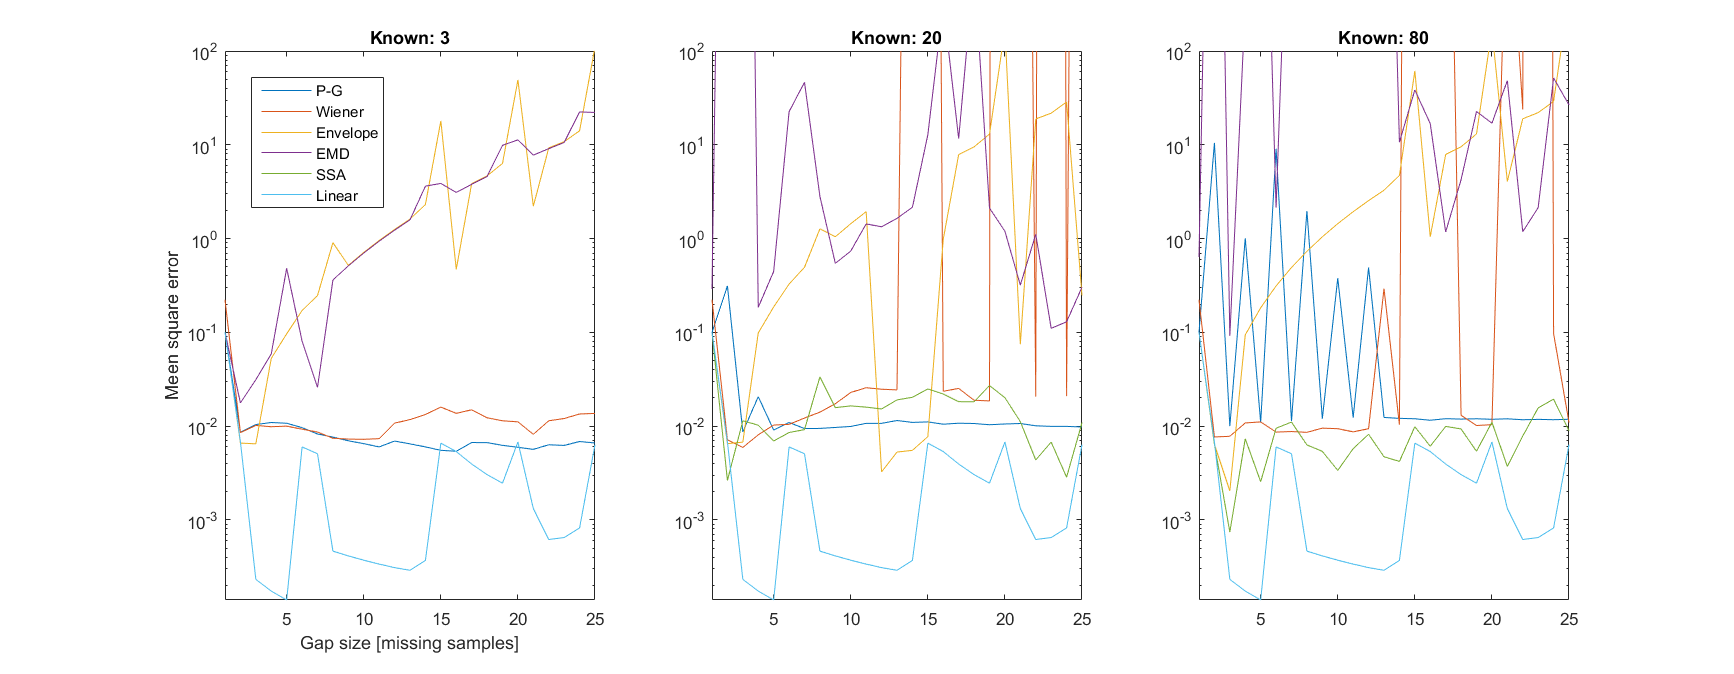
\includegraphics[width=1\textwidth]{billeder/RecJitter.png}
\caption{Jitter Power comparison of the reconstruction methods}
\label{fig:RecJit}
\end{figure}

As seen on figure \ref{fig:RecJit} does non of the methods model the noise very well, as is to be expected due to the nature of the selected methods. This is will probably not be a problem for the SmartHG data, since it is sampled at a very low sample rate, and noise therefore is not likely to be used as a parameter. For data there have been sampled with high frequency it have shown that the noise created by the different appliances can be used to detect them \citep{RefWorks:17}. 

\section{Chapter Discussion}
In the chapter the errors of the smartHG dataset is analysed. The dataset is a raw dataset, that have not undergone any cleaning prior to the process. It is shown that the most common errors in this types of data is single sample errors, and minor gaps of up to 5 missing samples.  

different kind of gap filling techniques is used on a series of artificial introduced gaps. It is shown that the small gaps, that are the most common, can be fixed relativity easy. For larger gaps it is harder do to, due to the stochastic nature of the signal. The stochastic element of a electric signal is often greater than the periodic part, which is a challenge for the gap filling. This combined with the low sample rate makes it hard to gesture about the true frequency content of the signal, since it is sampled way below the Nyquist rate.  
